\documentclass[]{article}
\usepackage{natbib}
\bibliographystyle{unsrtnat}
\usepackage{graphicx}
\usepackage{placeins}
\usepackage{url}
\graphicspath{ {./images/} }
\usepackage{wrapfig}
\renewcommand{\figurename}{Fig.}
%opening

\title{Identifying macro-moths with micro-features}
\author{Paul J. Palmer}

\begin{document}

\maketitle

\begin{abstract}

This article explores the use of external microscopic features to support the identification (ID) of  macro-lepidoptera. The usual process of identifying macro-moths often focusses on the wings, which are often large and distinctively patterned. Matching an unknown specimen to reference pictures is often the identification method employed given the lack of systematic keys for Lepidoptera in general and coupled with experience, can give good results. The article uses a problematic identification as an example of how microscopic features may be used to narrow the field of candidate taxa to arrive at a specific taxon. 

\end{abstract}

\section*{A Difficult Specimen to ID}
The specimen in question was taken at sugar 2020-08-16 on the Rutland Water Nature Reserve. It would have been recorded as a very worn example of \textit{Hypena proboscidalis} (The Snout) if it had not briefly raised its wings in a posture uncharacteristic for this species, placing an element of doubt in this presumption. As can be seen in Figure~\ref{fig:202009131026pjp-1}, the specimen lacks long, forward pointing palps that give the Snout its vernacular name, buts its wings have the same slightly hooked shape  and similar median fascia as the verified specimen illustrated in  Figure~\ref{fig:S202012271446-1}.  It would be easy to presume that the palps have been broken in what appears to be a worn specimen, but examination under magnification, as shown in  Figure~\ref{fig:20201112-1} reveals that the palps are short and undamaged. Less obvious, because it is less often mentioned in the descriptive text of guide books, is the lack of ocelli above the compound eye,  which effectively eliminates \textit{Hypena proboscidalis} as a candidate taxon for the specimen.

\section*{Finding an ID}
Dissection is always considered the definitive identification method, but a lack of keys means that other features must be used to reduce the pool of candidate species to a family and possibly genus otherwise we are back to matching pictures of dissections.  The matrix key published by \citet{Dombroskie2011} is intended for Canadian Lepidoptera, but can be used to provide an indicative guide to UK families too. Importantly, it is a useful indication of features that can be used to find the likely family of a specimen.

%In this case, although the specimen is a macro-moth, the family \textit{Erebidae}.
In this case, an examination of the head under magnification can help provide clues. 
The lack of oceli (simple eyes), coiled unscaled proboscis, and forward facing palps are suggestive of \textit{Geometridae}. The forewing length of 16.7 mm and the flight time of August are useful for eliminating many possible UK taxa.

\begin{figure}
	\centering
	\begin{minipage}{0.45\textwidth}
		\centering
	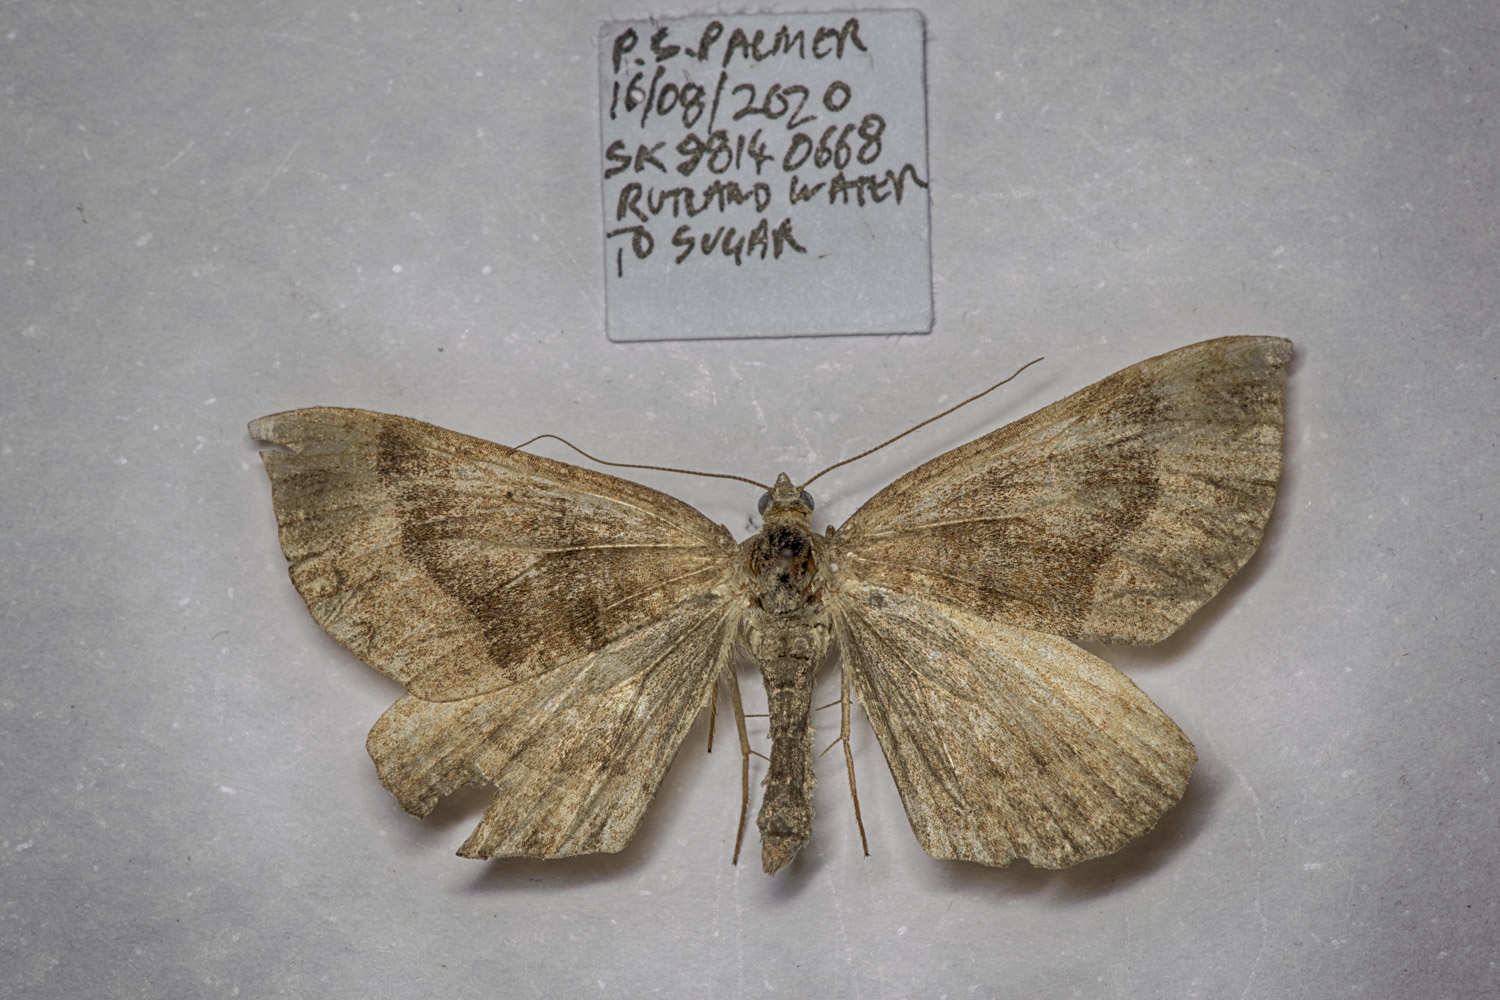
\includegraphics[width=0.9\linewidth]{images/202009131026PJP-1}
	\caption{The unkown specimen resembling Hypena proboscidalis.}
	\label{fig:202009131026pjp-1}
	\end{minipage}\hfill
	\begin{minipage}{0.45\textwidth}
		\centering
		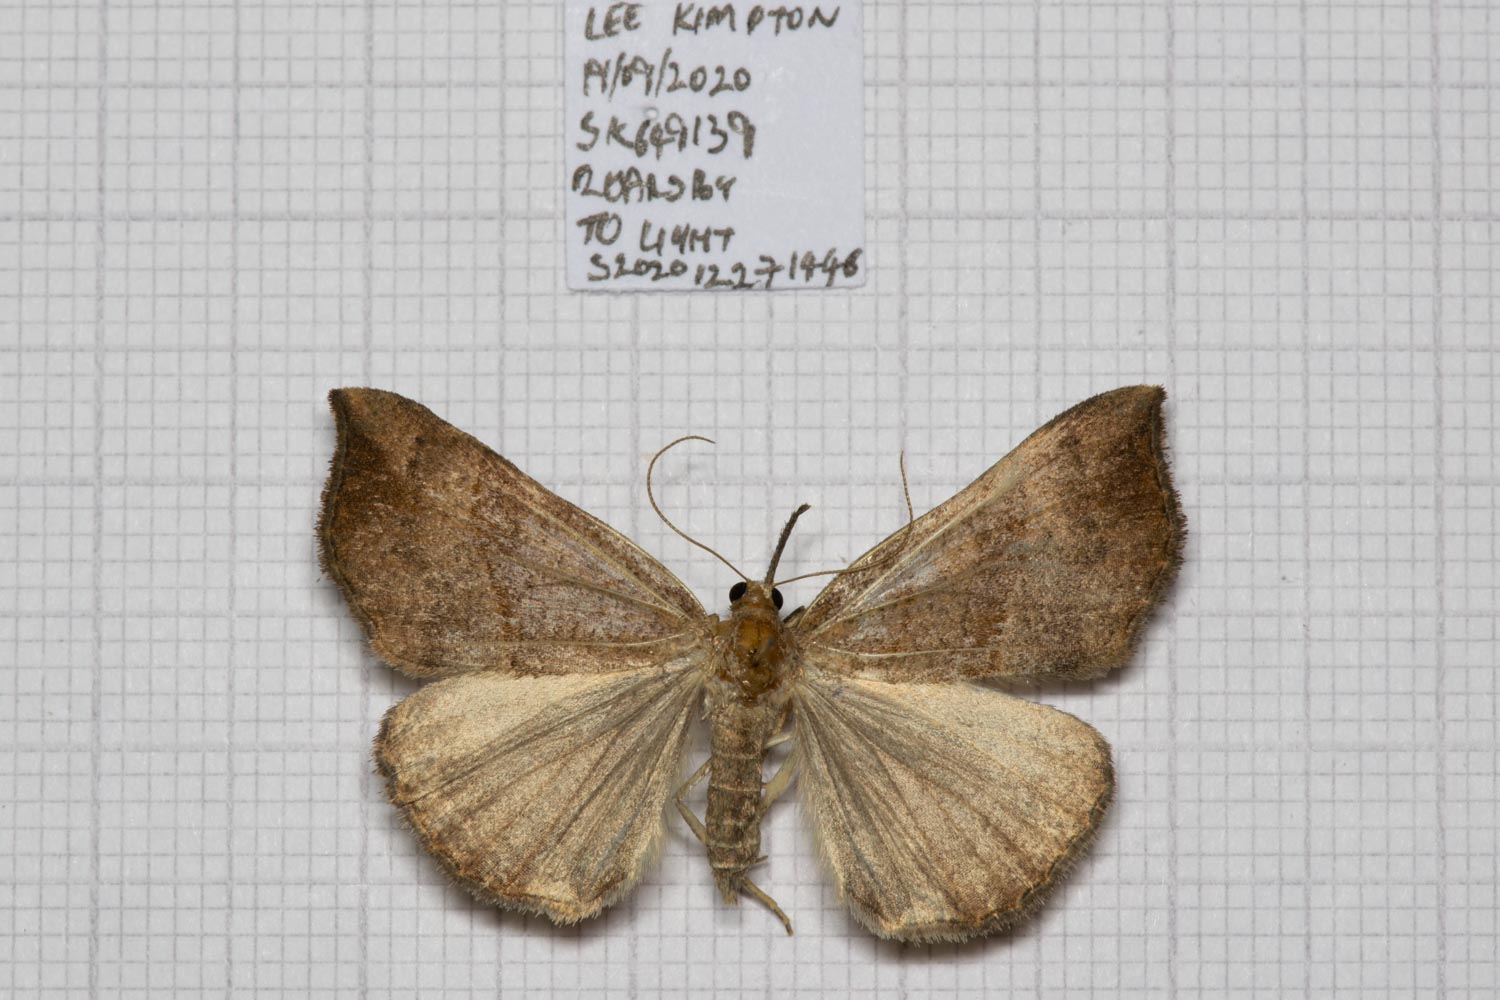
\includegraphics[width=0.9\textwidth]{S202012271446-1} % second figure itself
		\caption{A verified specimen of female Hypena proboscidalis.}
		\label{fig:S202012271446-1}
	\end{minipage}
\end{figure}



\begin{figure}
	\centering
	\begin{minipage}{0.45\textwidth}
		\centering
	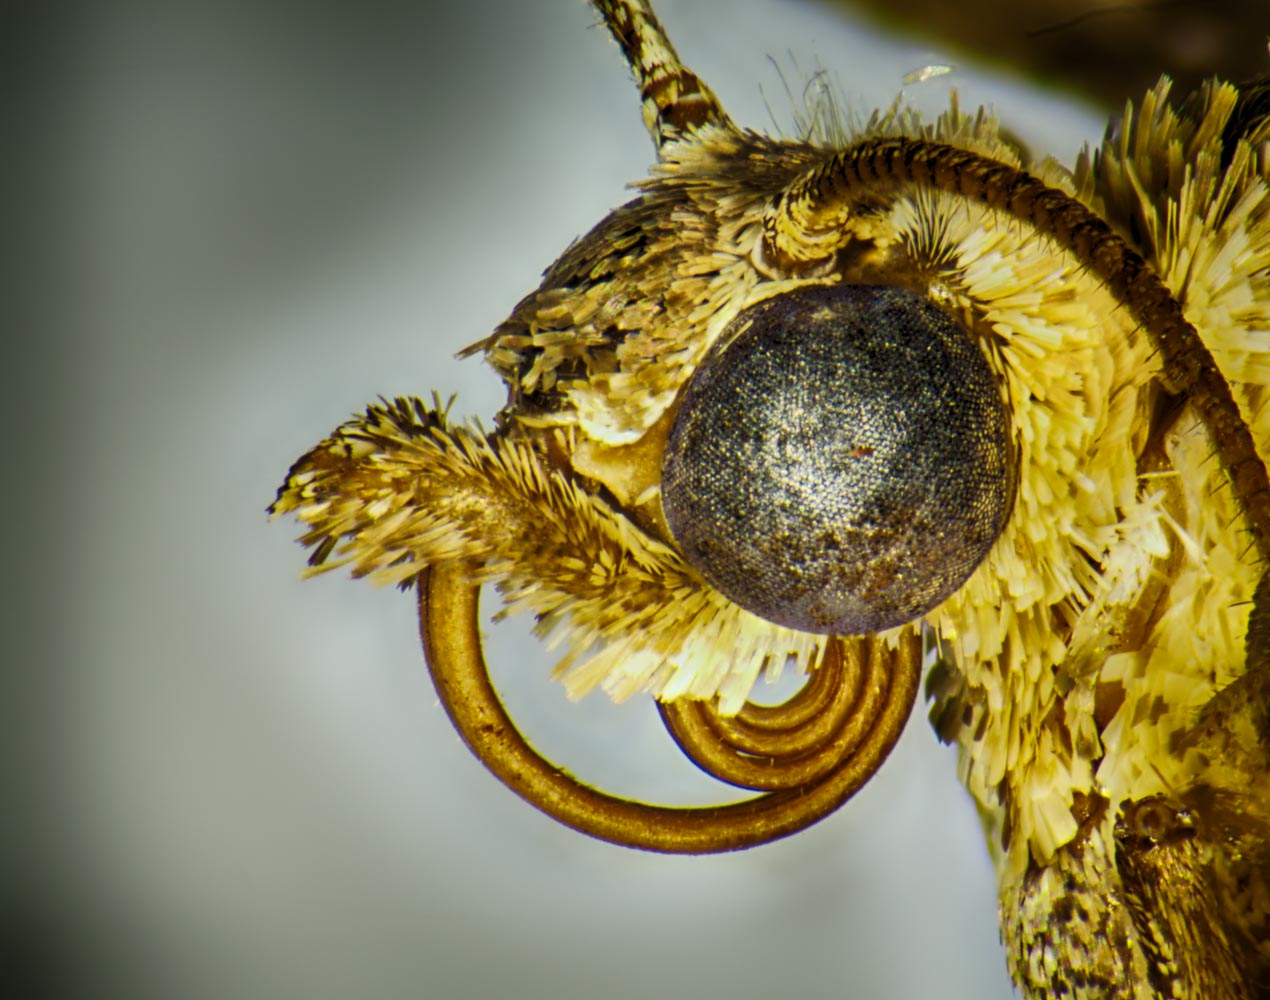
\includegraphics[width=0.5\linewidth]{images/20201112-1}
	\caption{Short undamaged palps eliminate Hypena proboscidalis as a candidate taxon.}
	\label{fig:20201112-1}
	\end{minipage}\hfill
	\begin{minipage}{0.45\textwidth}
		\centering
		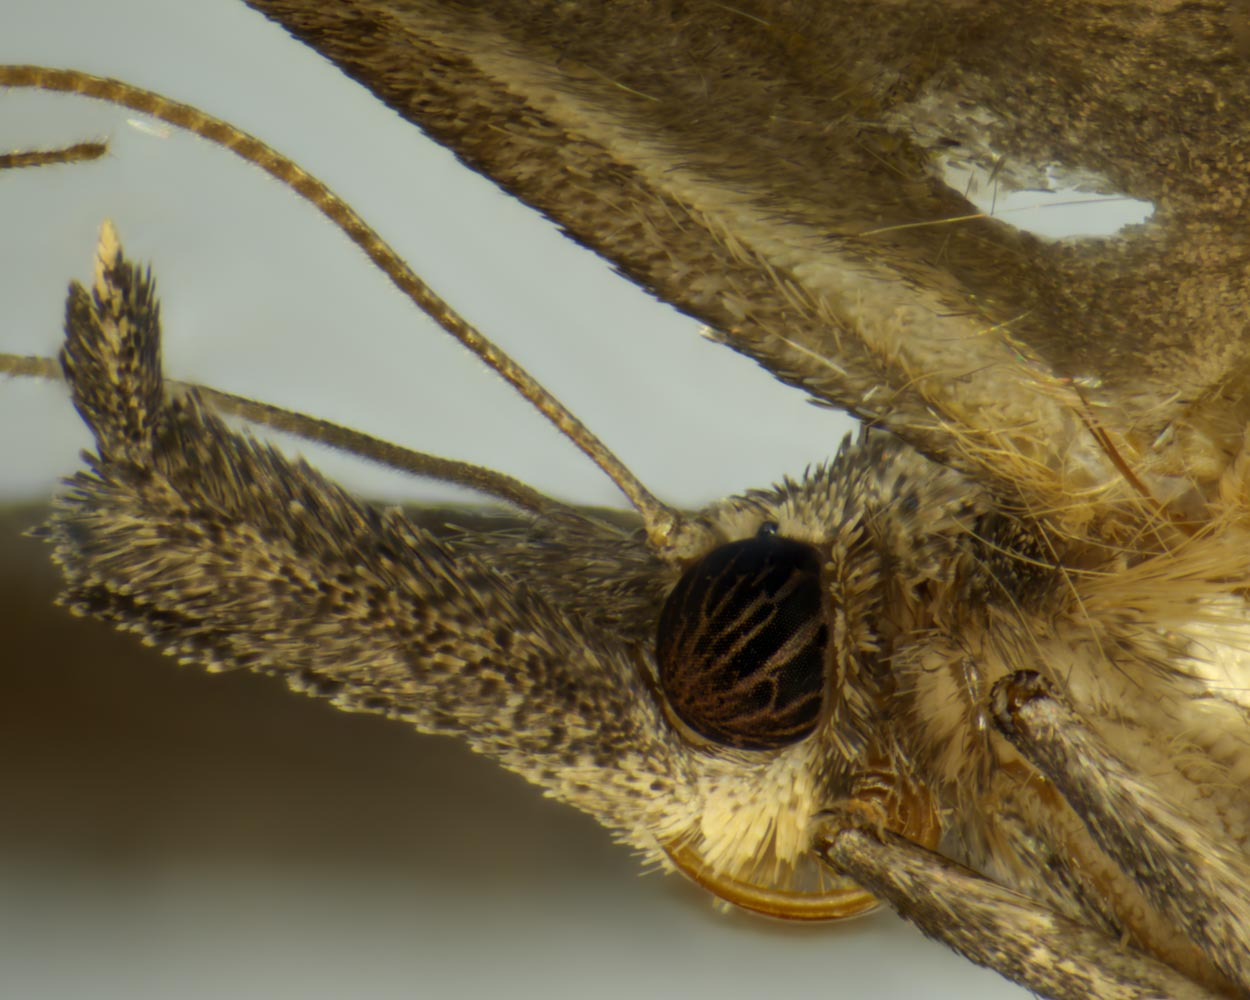
\includegraphics[width=0.9\textwidth]{S202012271446-4} % second figure itself
		\caption{Long, forward facing palps, and oceli above the compound eye of Hypena proboscidalis.}
		\label{fig:S202012271446-1}
	\end{minipage}
\end{figure}

%
%\begin{figure}
%	\centering
%	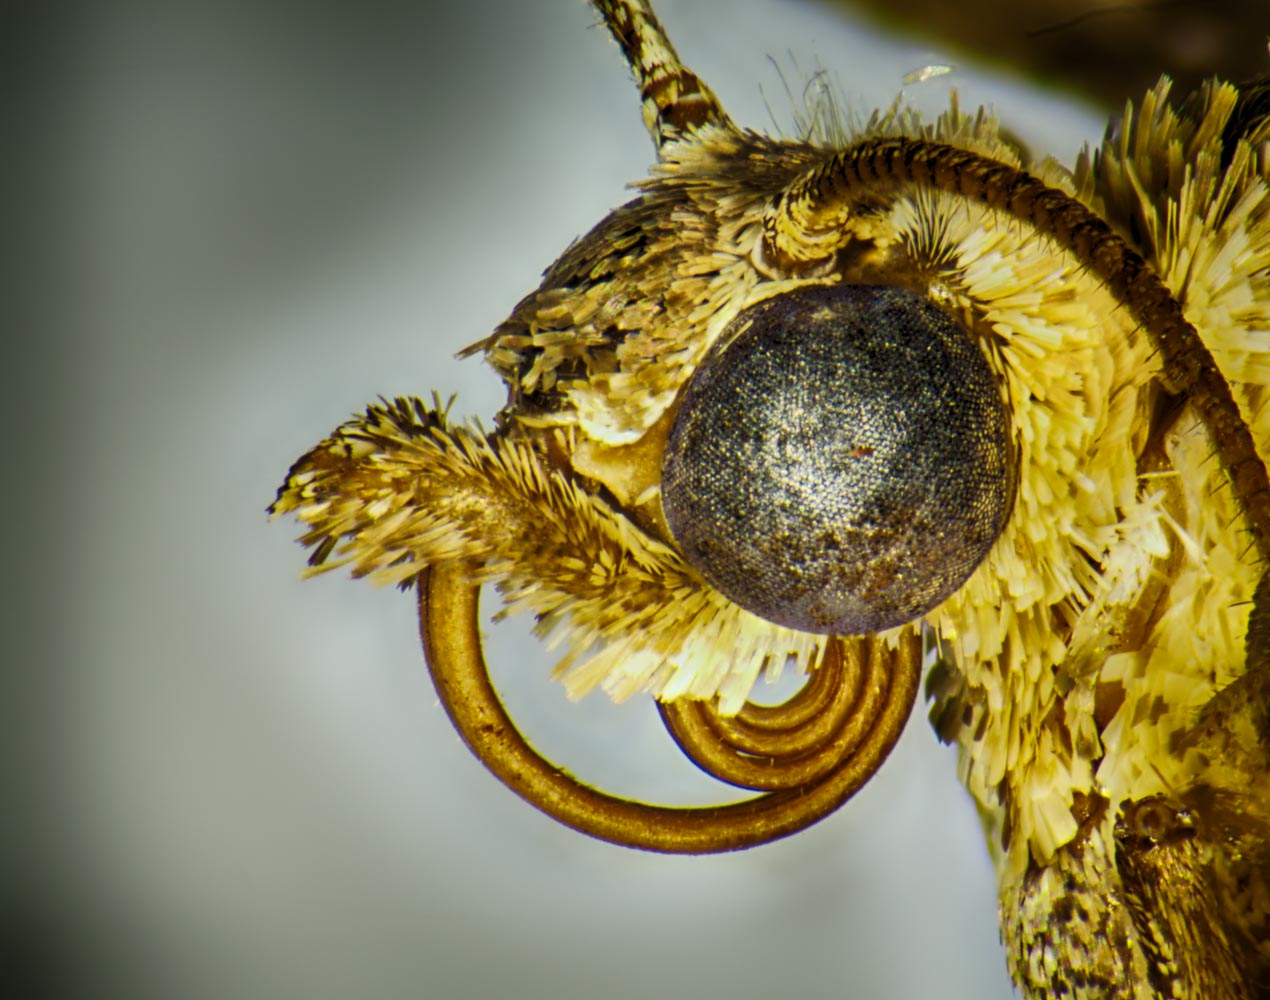
\includegraphics[width=0.5\linewidth]{images/20201112-1}
%	\caption{Short undamaged palps eliminate Hypena proboscidalis as a candidate taxon.}
%	\label{fig:20201112-1}
%\end{figure}


\bibliography{library}
\end{document}
